\href{}{}\documentclass[12pt,portuguese,oneside]{article}

%basico
\usepackage[portuguese]{babel}
\usepackage[T1]{fontenc}
\usepackage[utf8]{inputenc}
\usepackage{float}

%fonte
\usepackage{newtxtext,newtxmath}

\usepackage{tabularx}
\usepackage[table]{xcolor}
\usepackage{caption}
\captionsetup[table]{skip=5pt}

\usepackage{longtable}
\usepackage{booktabs}
\usepackage[margin=2.5cm]{geometry} % ajuste a margem conforme necessário



% aparencia
\usepackage{graphicx}
\usepackage{geometry}
\usepackage{setspace}
\usepackage{titlesec}
\usepackage{fancyhdr}
\usepackage{tocloft}
\usepackage{natbib}
\usepackage{amsmath}

% margens
\geometry{
  top=3cm,
  bottom=2cm,
  left=3cm,
  right=2cm,
}

% espaçamento entre linhas
\onehalfspacing

% recuo automático
\setlength{\parindent}{1.5em}

% estilo de seções
\titleformat{\section}[block]{\fontsize{12}{15}\selectfont\bfseries}{\thesection}{0.5cm}{}
\titleformat{\subsection}[block]{\fontsize{12}{15}\selectfont\bfseries}{\thesubsection}{0.5cm}{}
\titleformat{\subsubsection}[block]{\fontsize{12}{15}\selectfont\itshape\bfseries}{\thesubsubsection}{1em}{}

% sumário espaçado
\setlength{\cftbeforesecskip}{4pt}

\pagestyle{fancy}
\fancyhf{} 
\fancyhead[C]{
\includegraphics[width=1cm]{imagens/logo.png}} % logo centralizada 
\renewcommand{\headrulewidth}{0.7pt} % linha do cabeçalho
\setlength{\headsep}{1.5cm}

%tabela
\usepackage{longtable}

\begin{document}


\begin{center}
  \fontsize{12}{12}\selectfont\textbf{UNIVERSIDADE FEDERAL DA FRONTEIRA SUL - \textit{CAMPUS} CHAPECÓ \\
  CURSO DE BACHAREL EM CIÊNCIA DA COMPUTAÇÃO \\
  ENGENHARIA DE SOFTWARE I \\
  DOCENTE: PROFª DRª RAQUEL APARECIDA PEGORARO \\}
\end{center}

\begin{center}
  \vspace*{3cm}
  {\fontsize{12}{12}\selectfont\bfseries\uppercase{CAROLINE DE QUADROS PIAZZA E MAIQUELI EDUARDA DAMA MINGOTI}} \\
  \vspace{1cm} 
  \vfill
\end{center}

\begin{center}
  \vspace*{1cm}
  {\fontsize{12}{12}\selectfont\bfseries\uppercase{Trabalho Integrador:}} \\
  {\fontsize{12}{12}\selectfont\uppercase{Descrição sobre a empresa e Elicitação}} \\
  \vspace{8cm} 
\today
  \vfill
\end{center}


\newpage
\selectlanguage{portuguese}
\renewcommand{\contentsname}{SUMÁRIO}
\renewcommand{\cfttoctitlefont}{\normalsize\bfseries}
\tableofcontents

\newpage

\section{EMPRESA}

\subsection{Apresentação da empresa}

\hspace{1em}O Instituto EDMA é uma clínica localizada no município de Chapecó, estado de Santa Catarina, com atuação voltada à prática clínica integrativa, centrada na prescrição e acompanhamento terapêutico com fitocanabinoides. A instituição atende pacientes em modalidade presencial e remota, com foco em intervenções individualizadas baseadas em evidências clínicas. Os atendimentos presenciais são realizados em Chapecó, na Av. Getúlio Dorneles Vargas, 180S - sala 26 - Centro.

A dinâmica de atendimento envolve três etapas principais: (1) triagem inicial, por meio de formulário estruturado de anamnese; (2) consulta clínica, com duração média de 40 a 60 minutos, em que se realiza uma avaliação detalhada do histórico de vida, queixas principais, rotina, uso de medicações e fatores psicossociais; e (3) acompanhamento clínico por 90 dias, com suporte contínuo para ajustes terapêuticos, conforme a evolução sintomática.

As condições mais frequentemente tratadas incluem transtornos de ansiedade, insônia, dor crônica, transtorno do déficit de atenção com hiperatividade (TDAH), doenças autoimunes, condições neurodegenerativas e cuidados complementares no contexto oncológico. O Instituto também acompanha atletas de alto rendimento, com demandas relacionadas à recuperação física, qualidade do sono e modulação de processos inflamatórios.

As condutas clínicas seguem o princípio de escalonamento gradual de dose (“start low, go slow”), com uso de formulações isoladas (CBD, THC, CBG), broad spectrum (sem THC) e full spectrum (com fitocomplexo completo). A escolha das formulações considera o perfil clínico, a rotina, os objetivos terapêuticos e a sensibilidade do paciente aos canabinoides.

A instituição não realiza a comercialização de produtos, limitando-se à orientação clínica quanto à escolha de marcas que atendam critérios de qualidade, rastreabilidade, transparência e conformidade com a legislação vigente. O monitoramento da evolução clínica é realizado com apoio de planilhas de acompanhamento preenchidas pelos pacientes, e a comunicação ocorre, preferencialmente, via Whatsapp.


\subsection{Nome da(s) pessoa(s) entrevista(s) e função/cargo}
\hspace{1em}A coleta de dados foi realizada junto a uma profissional da equipe clínica e quatro pacientes em acompanhamento no Instituto EDMA.

A profissional entrevistada foi Brunna Varela, biomédica responsável pelos atendimentos clínicos e pela prescrição dos óleos de cannabis no Instituto. Sua atuação abrange desde a triagem inicial dos pacientes até a condução do tratamento, incluindo a seleção da formulação mais adequada, orientações de uso, monitoramento dos efeitos terapêuticos e realização de ajustes individualizados conforme a resposta clínica.

\begin{figure}[H]
    \centering
    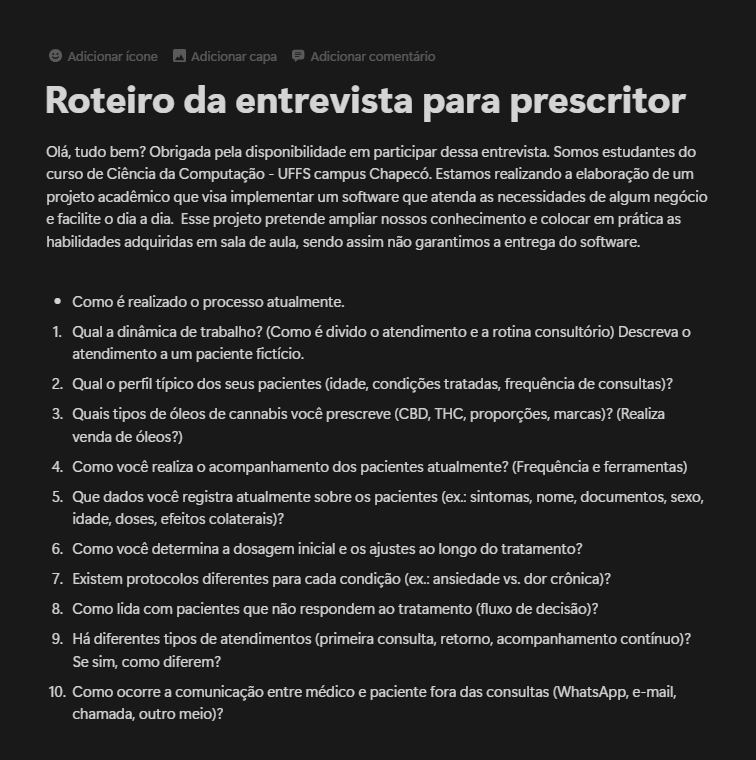
\includegraphics[width=0.4\linewidth]{imagens/roteiro1.png}
    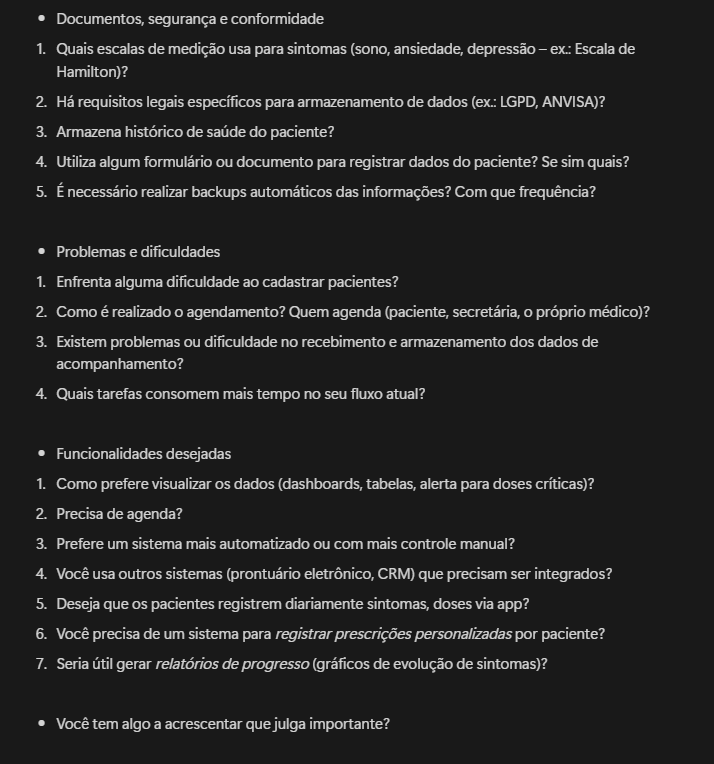
\includegraphics[width=0.4\linewidth]{imagens/roteiro2.png}
    \caption{Roteiro da entrevista com a preescritora. Registro do Autor (2025).}
    \label{fig:roteiro.png}
\end{figure}

Além da profissional, participaram da elicitação quatro pacientes em acompanhamento no Instituto EDMA, os quais responderam a um formulário eletrônico encaminhado diretamente pela prescritora. Os participantes apresentaram as seguintes características:

- Idades: 25, 30, 32 e 42 anos;

- Principais condições relatadas: ansiedade, convulsões, inflamações (como acne) e uso com finalidade geral de promoção da qualidade de vida, sem presença de doença diagnosticada.

As respostas indicaram variações na frequência de contato com a prescritora (de consultas mensais a retornos apenas quando necessário), nas estratégias utilizadas para lembrar os horários de administração (rotina, memória, local de acesso visual), e nos métodos de acompanhamento do tratamento (anotações manuais, aplicativos, anotações digitais não especializadas). Também foram apontadas preferências por dispositivos móveis para registro e consulta de informações, além do interesse em funcionalidades adicionais, como lembretes de dose e espaços de relato entre consultas.

\begin{figure}[H]
    \centering
    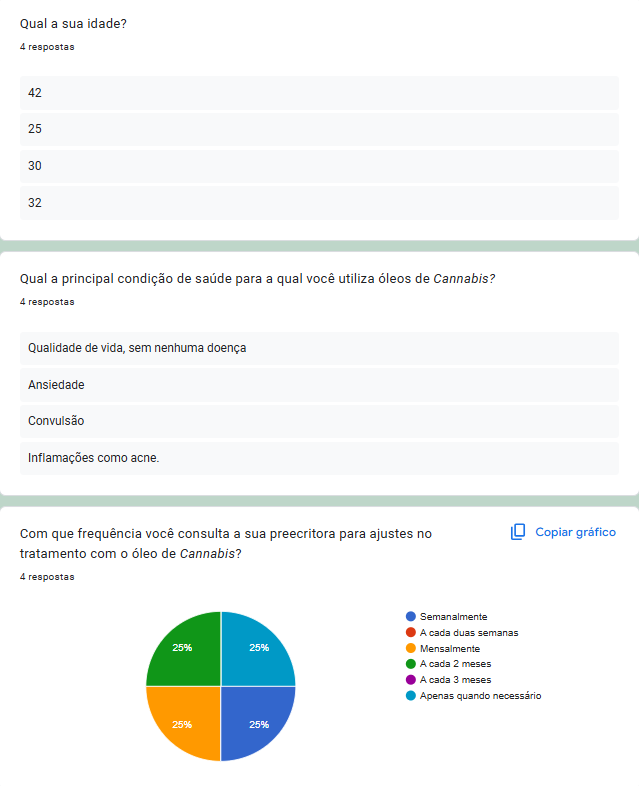
\includegraphics[width=0.4\linewidth]{imagens/forms1.png}
    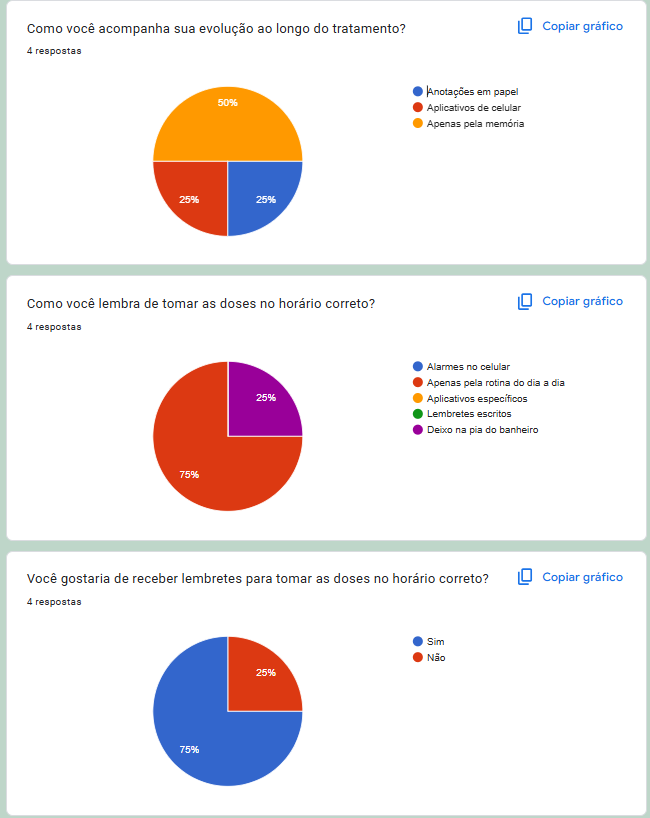
\includegraphics[width=0.4\linewidth]{imagens/forms2.png}
    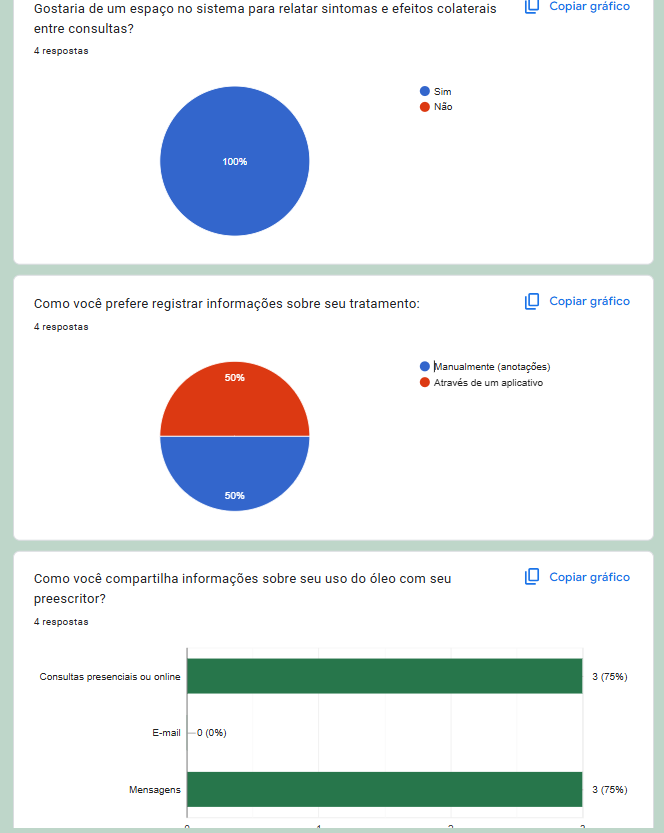
\includegraphics[width=0.4\linewidth]{imagens/forms3.png}
    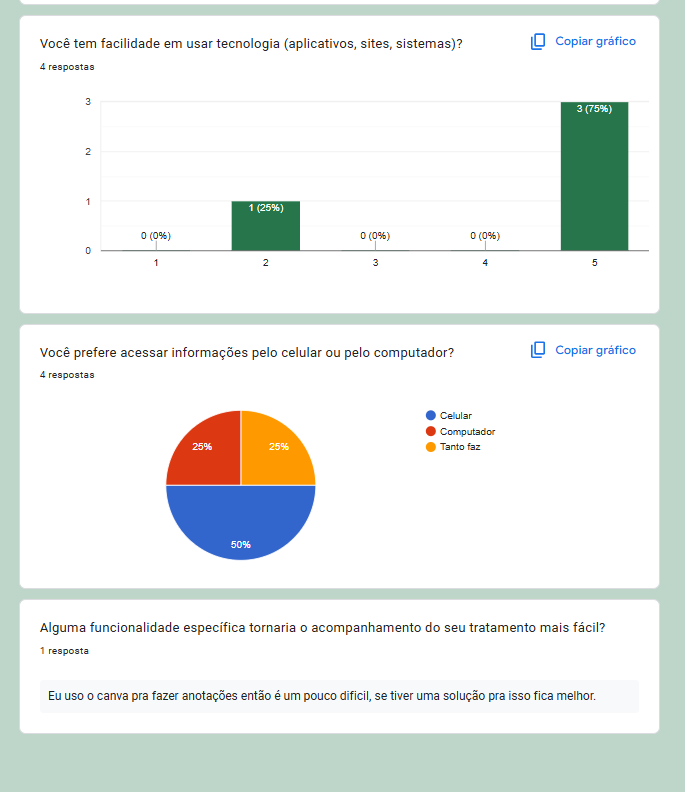
\includegraphics[width=0.4\linewidth]{imagens/forms4.png}
    \caption{Formulário com respostas dos pacientes. Registro do Autor (2025).}
    \label{fig:roteiro.png}
\end{figure}

\subsection{Descrição do funcionamento da empresa}

\hspace{1em}

O Instituto EDMA atua com foco em atendimentos clínicos voltados à prescrição de fitocanabinoides, fundamentados em uma abordagem integrativa e centrada no paciente. O funcionamento da clínica está organizado em um fluxo que compreende três etapas principais: triagem inicial, consulta clínica e acompanhamento terapêutico.

A triagem é realizada previamente à primeira consulta, por meio do envio de um formulário estruturado de anamnese. Esse documento é preenchido pelo paciente e contém informações clínicas, psicossociais, histórico de uso de medicações, diagnósticos anteriores e queixas principais. Os dados coletados são registrados manualmente e inseridos no prontuário eletrônico utilizado pela clínica.

\begin{figure}[H]
    \centering
    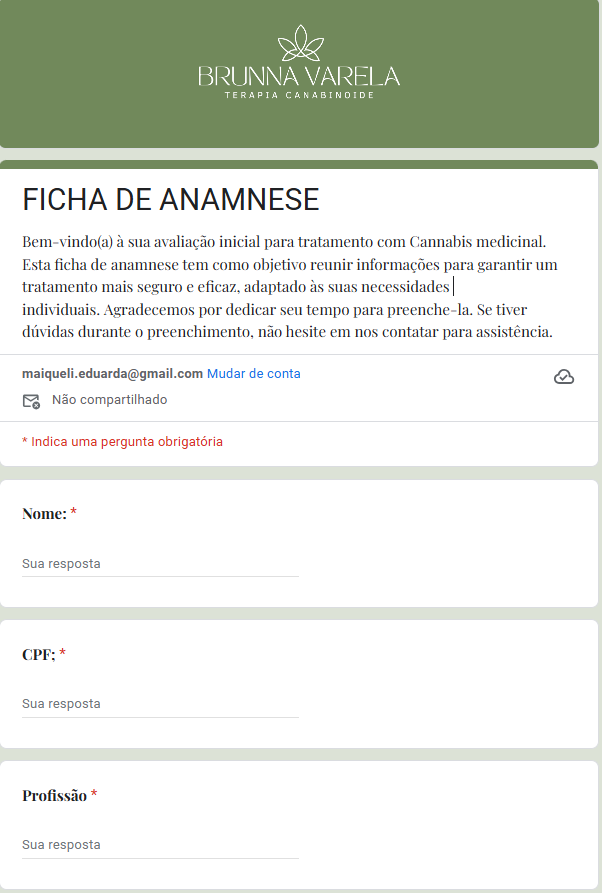
\includegraphics[width=0.4\linewidth]{imagens/anamnese1.png}
    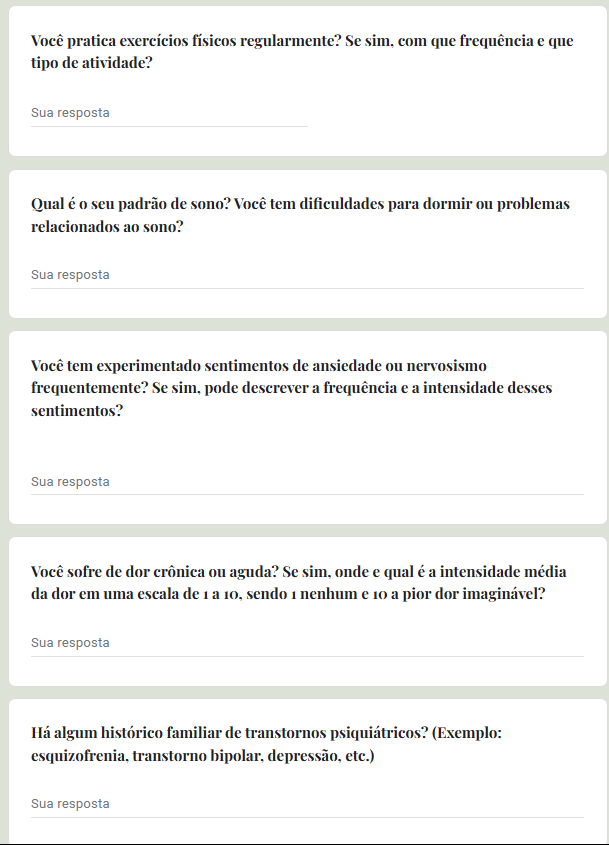
\includegraphics[width=0.4\linewidth]{imagens/anamnese2.png}
    \caption{Ficha de Anamnese. Registro do Autor (2025).}
    \label{fig:anamnese.png}
\end{figure}

Após a triagem, é agendada a consulta clínica, com duração média de 40 a 60 minutos. Durante esse atendimento, a profissional responsável realiza uma avaliação detalhada, com base no histórico de vida do paciente, rotina, perfil emocional e objetivos terapêuticos. Com base nessa análise, define-se a estratégia terapêutica inicial, incluindo a escolha da formulação (isolada, broad ou full spectrum) e o protocolo de escalonamento da dose, seguindo o princípio de início com baixa dosagem e aumento progressivo conforme a resposta individual.

O acompanhamento clínico é realizado ao longo de 90 dias, período no qual o paciente deve relatar sua evolução, sintomas, possíveis efeitos adversos e demais observações relevantes. Esse acompanhamento é feito por meio de contatos semanais, majoritariamente via WhatsApp, e por planilhas de controle que são preenchidas pelos próprios pacientes. Os dados gerados nesse período são posteriormente migrados manualmente para o prontuário.

\begin{figure}[H]
    \centering
    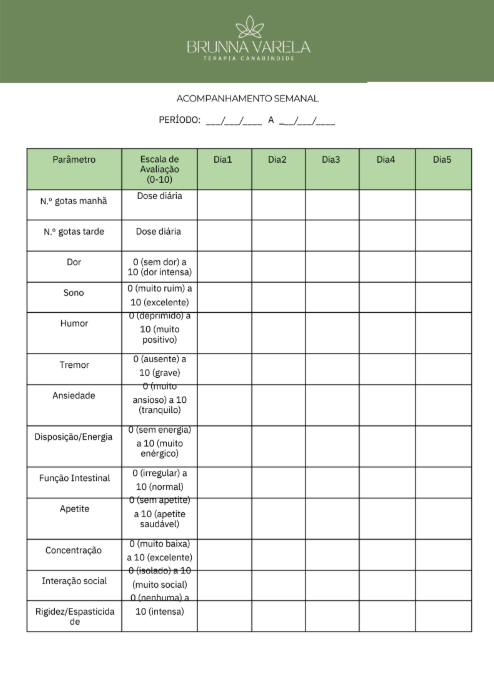
\includegraphics[width=0.4\linewidth]{imagens/acompanhamento1.png}
    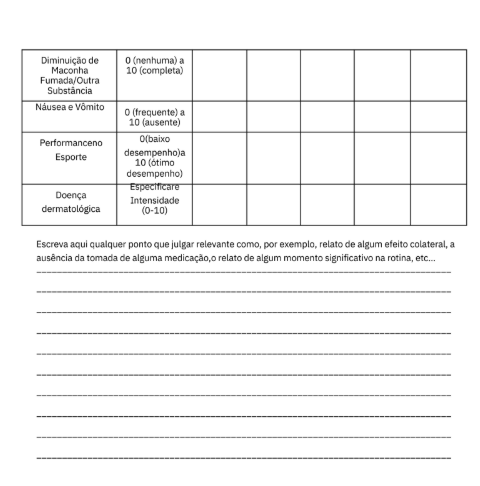
\includegraphics[width=0.4\linewidth]{imagens/acompanhamento2.png}
    \caption{Acompanhamento semanal. Registro do Autor (2025).}
    \label{fig:acompanhamento.png}
\end{figure}

O agendamento de consultas e organização do fluxo de pacientes são realizados pela própria prescritor(a), sem apoio de equipe administrativa. O processo de cadastro de novos pacientes e coleta inicial de informações ainda não é automatizado, o que acarreta acúmulo de tarefas operacionais.

Quanto ao armazenamento de dados clínicos, a clínica faz uso de diferentes sistemas: formulários digitais, planilhas locais e mensagens em aplicativos de troca de mensagens. O prontuário eletrônico em uso está em processo de migração para a plataforma Amplimed, uma vez que o sistema anterior, voltado à área de estética, mostrou-se inadequado às demandas clínicas específicas.

Por fim, é relevante destacar que a clínica adota escalas clínicas padronizadas para algumas condições específicas, como a Escala de Hamilton (ansiedade), o Índice de Qualidade do Sono de Pittsburgh, o Mini-Mental (para triagem cognitiva) e, eventualmente, outras escalas obtidas de parceiros da área laboratorial. No entanto, a aplicação dessas ferramentas é limitada pela baixa adesão de parte dos pacientes ao preenchimento regular das mesmas.
\begin{figure}[H]
    \centering
    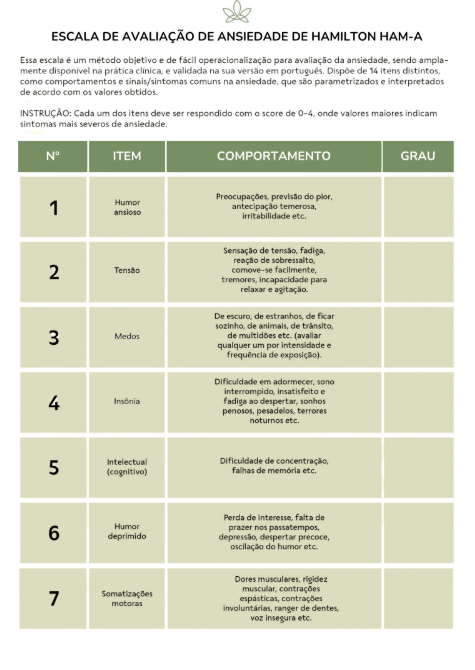
\includegraphics[width=0.4\linewidth]{imagens/ansiedade1.png}
    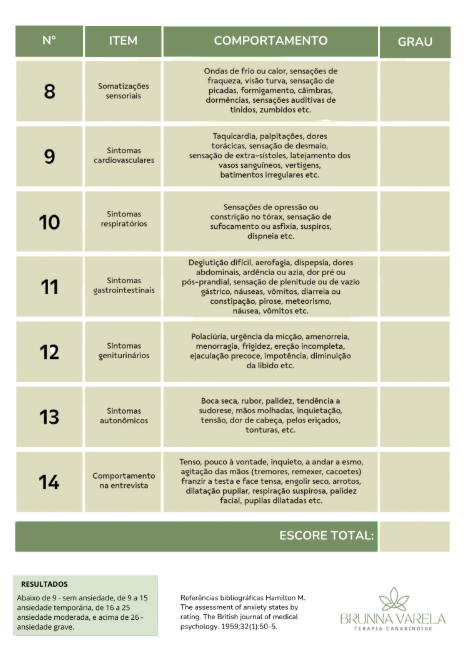
\includegraphics[width=0.4\linewidth]{imagens/ansiedade2.png}
    \caption{Escala de Hamilton para ansiedade. Registro do Autor (2025).}
    \label{fig:ansiedade.png}
\end{figure}
\begin{figure}[H]
    \centering
    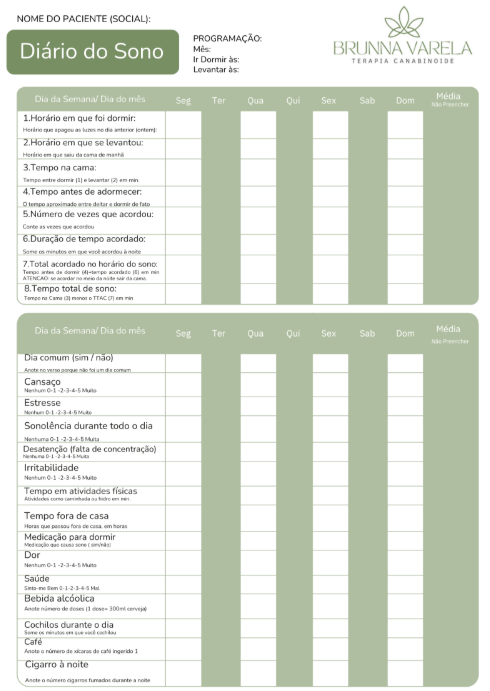
\includegraphics[width=0.4\linewidth]{imagens/sono.png}
    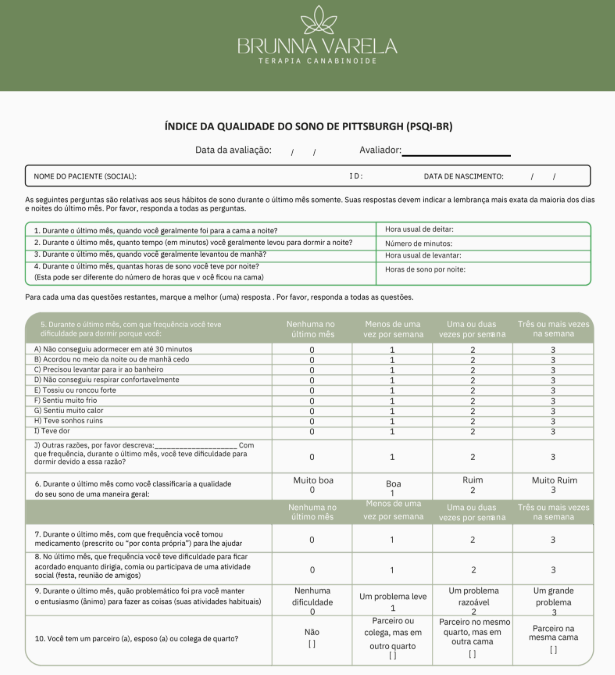
\includegraphics[width=0.4\linewidth]{imagens/qualidadesono.png}
    \caption{Acompanhamento e escala da qualidade do sono. Registro do Autor (2025).}
    \label{fig:sono.png}
\end{figure}

\begin{figure}[H]
    \centering
    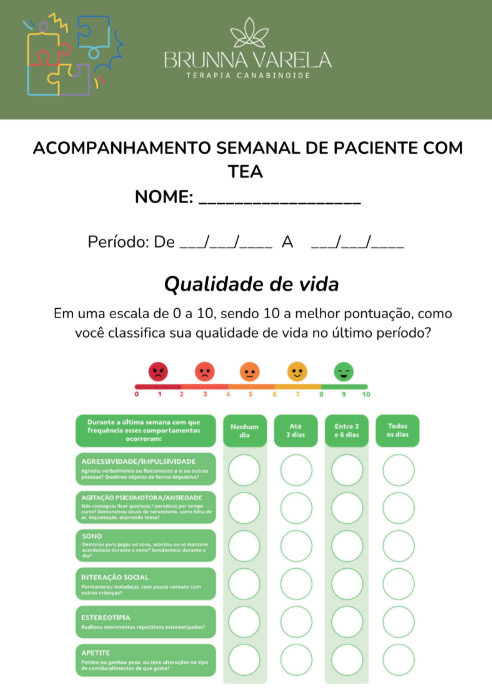
\includegraphics[width=0.4\linewidth]{imagens/tea.png}
    \caption{Acompanhamento semanal de paciente com TEA. Registro do Autor (2025).}
    \label{fig:tea.png}
\end{figure}
\begin{figure}[H]
    \centering
    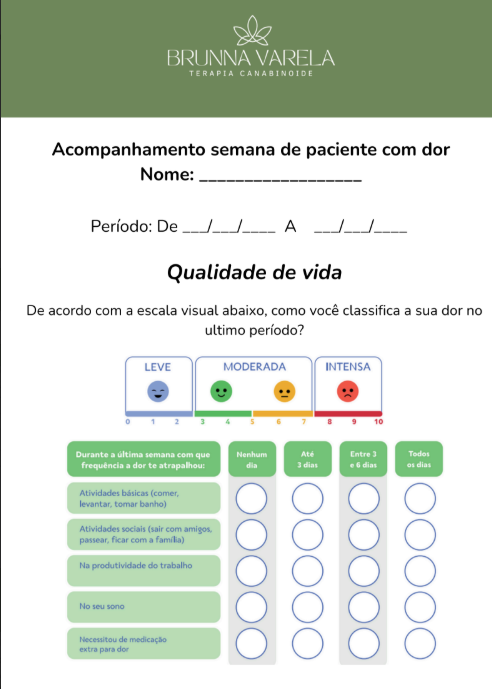
\includegraphics[width=0.4\linewidth]{imagens/dor.png}
    \caption{Acompanhamento semanal de paciente com Dor. Registro do Autor (2025).}
    \label{fig:dor.png}
\end{figure}
\begin{figure}[H]
    \centering
    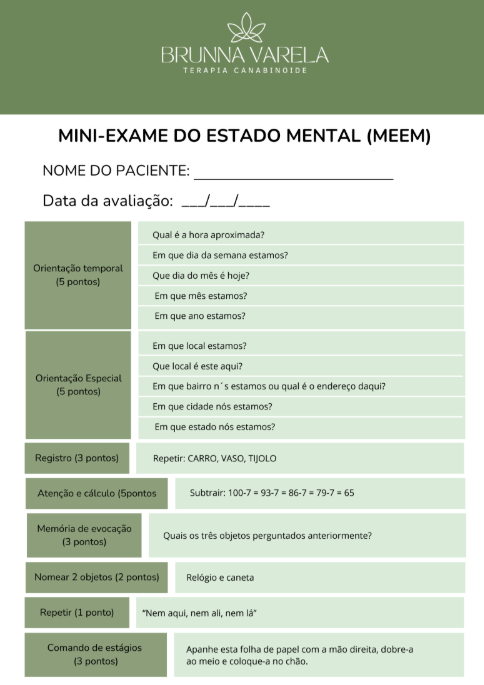
\includegraphics[width=0.4\linewidth]{imagens/meem.png}
    \caption{Mini-exame do estado mental (MEEM). Registro do Autor (2025).}
    \label{fig:meem.png}
\end{figure}

\begin{figure}[H]
    \centering
    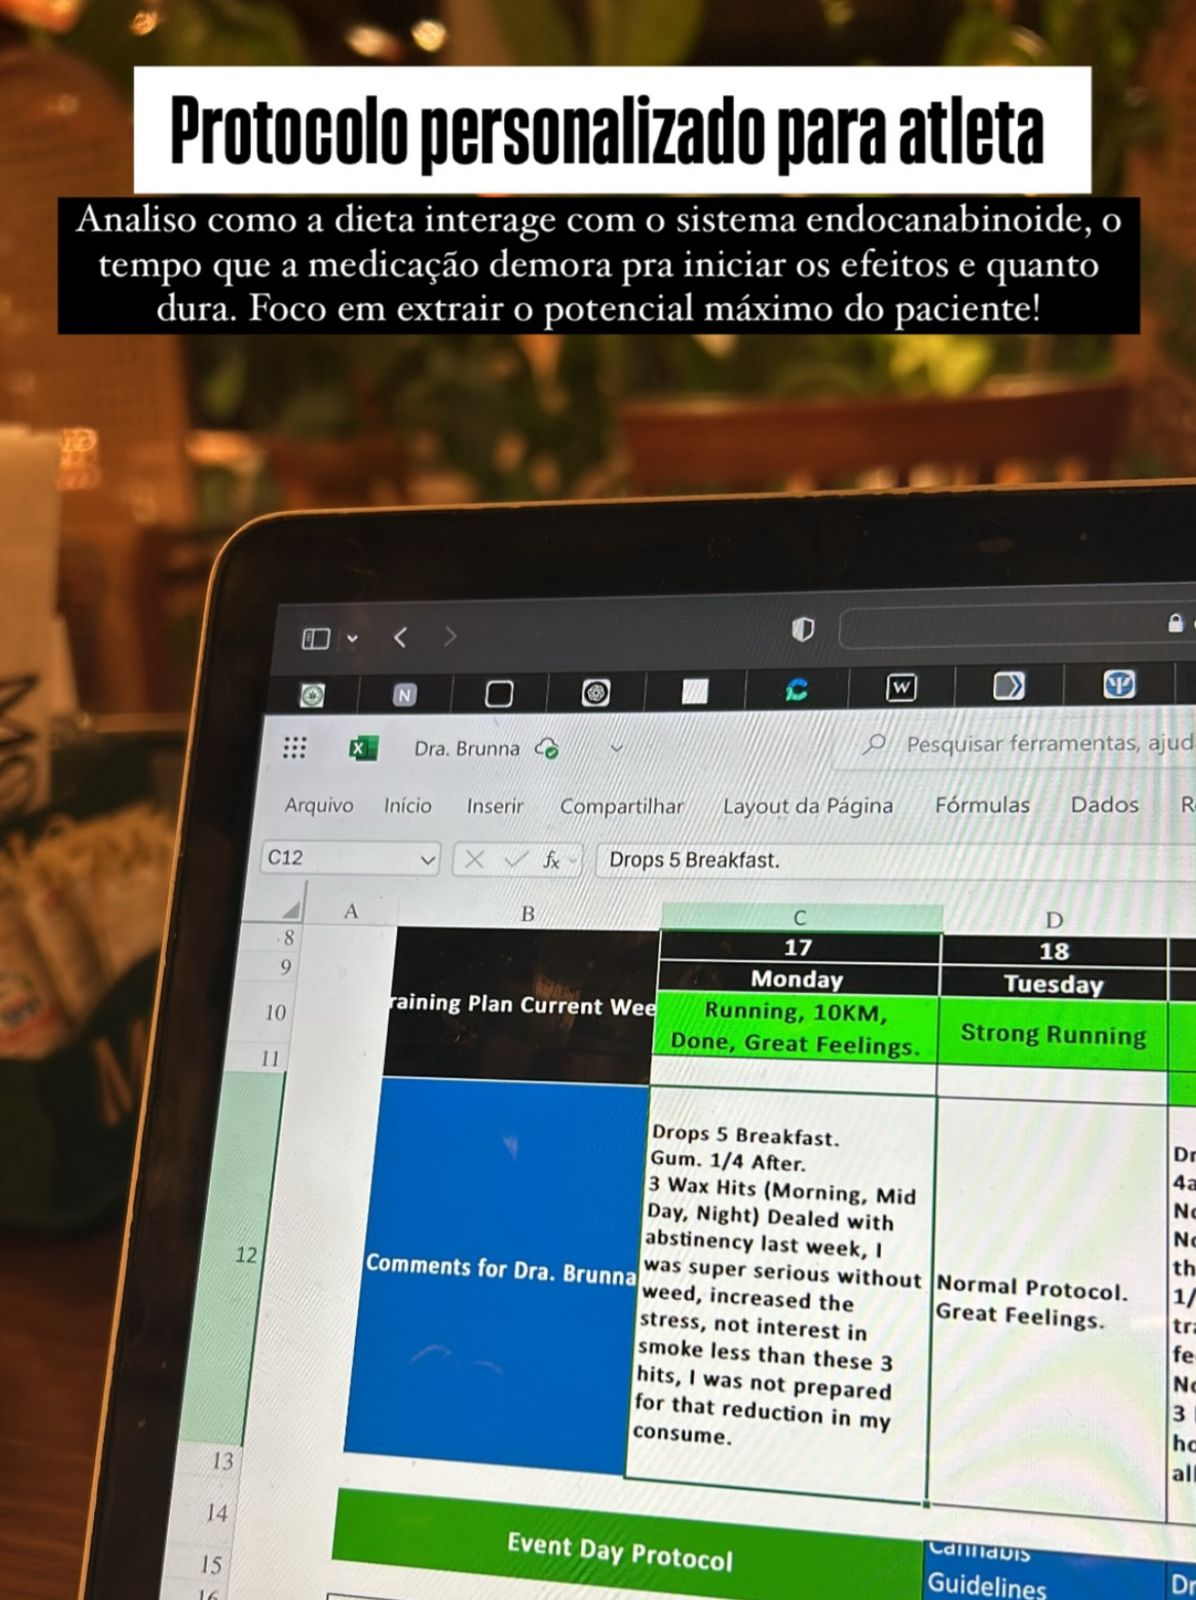
\includegraphics[width=0.4\linewidth]{imagens/atleta.jpeg}
    \caption{Ficha personalizada para atletas. Registro do Autor (2025).}
    \label{fig:atleta.png}
\end{figure}


\subsection{Problemas e/ou desafios enfrentados}
\hspace{1em}Durante a entrevista com a profissional responsável pelo Instituto EDMA, foram identificados diversos desafios relacionados ao funcionamento atual da clínica, abrangendo desde questões operacionais até limitações nos processos de gestão de dados clínicos e acompanhamento terapêutico. As dificuldades observadas comprometem a eficiência do serviço, a qualidade do monitoramento dos pacientes e a capacidade de escalabilidade da instituição.

O primeiro desafio relevante refere-se à ausência de automação nos processos internos. Atualmente, grande parte do fluxo de trabalho é executado manualmente, incluindo etapas como o cadastro de novos pacientes, envio e recebimento de formulários, preenchimento de dados clínicos e atualização dos prontuários eletrônicos. Essas atividades são realizadas integralmente pela profissional clínica, que também acumula funções administrativas, como agendamento de consultas, triagem de pacientes e transcrição de informações obtidas nas entrevistas. Essa centralização de tarefas provoca uma sobrecarga significativa, aumentando o risco de erros, atrasos e perda de dados clínicos importantes.

Outro problema recorrente diz respeito à comunicação descentralizada e não estruturada com os pacientes. A principal ferramenta de contato utilizada é o aplicativo WhatsApp, que, apesar de prático, não permite o registro formal, sistemático e integrado das informações trocadas. Isso implica em retrabalho constante, já que os dados precisam ser manualmente migrados para o prontuário eletrônico, processo que demanda tempo e está sujeito a falhas, omissões ou inconsistências no histórico clínico.

A baixa adesão dos pacientes às ferramentas de acompanhamento terapêutico também foi apontada como um fator limitante. O acompanhamento depende do preenchimento voluntário de planilhas ou do envio espontâneo de mensagens pelos próprios pacientes. No entanto, foi relatado um baixo engajamento por parte do público atendido, o que compromete a regularidade e a qualidade dos dados coletados entre as consultas. A falta de um sistema automatizado ou de notificações regulares torna o processo menos atrativo e dificulta a continuidade do monitoramento clínico.

Outro ponto crítico é a falta de integração entre as ferramentas utilizadas no dia a dia da clínica. As sistemas em uso, como WhatsApp, Google Forms, planilhas do Google e o sistema de prontuário eletrônico, operam de forma isolada, sem qualquer interoperabilidade. Essa fragmentação prejudica a rastreabilidade dos dados, dificulta a geração de relatórios clínicos e inviabiliza a sistematização de informações para fins científicos, o que é especialmente relevante em se tratando de uma prática terapêutica baseada em evidências.

Adicionalmente, foram destacadas limitações do sistema de prontuário eletrônico atualmente em uso. A clínica iniciou recentemente a migração para o sistema Amplimed, após tentativas malsucedidas com outras sistemas que não atendiam às especificidades da prática clínica com fitocanabinoides. Embora o novo sistema represente um avanço, ele ainda está em fase de adaptação e não contempla funcionalidades consideradas essenciais, como o envio automatizado de formulários periódicos, a integração com dashboards analíticos personalizados e o registro estruturado de dados sintomáticos e terapêuticos.

Por fim, a clínica enfrenta a ausência de apoio administrativo. Todas as atividades administrativas permanecem sob responsabilidade direta da profissional clínica, incluindo o atendimento inicial, controle de agenda, preenchimento de prontuários, coleta de informações e acompanhamento pós-consulta. Essa ausência de apoio humano ou de automação tecnológica agrava ainda mais a sobrecarga de trabalho e limita a capacidade de expansão da clínica, impedindo o aumento do número de atendimentos ou a diversificação dos serviços oferecidos.

Assim, os desafios enfrentados pelo Instituto EDMA refletem a necessidade urgente de um sistema informatizado, integrado e responsivo, que otimize os fluxos operacionais, melhore a qualidade do atendimento e reduza o esforço manual envolvido na rotina clínica.


\subsection{Necessidades e/ou expectativas para o novo sistema}

\hspace{1em} Sob a perspectiva da profissional prescritor(a), uma das principais necessidades identificadas refere-se à automação e integração das etapas do processo clínico. Atualmente, a maior parte das tarefas é realizada de forma manual ou com uso de ferramentas não integradas, o que compromete a eficiência operacional, aumenta o risco de inconsistência de dados e exige tempo excessivo para execução de atividades repetitivas. Dentre as funcionalidades prioritárias, destaca-se a necessidade de um sistema que permita o cadastro automático de novos pacientes por meio de formulários digitais, que otimize o processo de triagem inicial e elimine etapas redundantes. Além disso, é essencial que o sistema integre os dados da triagem com a agenda da profissional, o prontuário eletrônico e os registros do acompanhamento clínico, permitindo acesso unificado às informações de cada paciente.

Outro aspecto relevante identificado na entrevista com a prescritor(a) é a necessidade de ferramentas para o acompanhamento clínico contínuo. A profissional apontou a importância de enviar formulários semanais padronizados para os pacientes, a fim de coletar dados sobre sintomas, efeitos colaterais e evolução terapêutica. Esses dados devem ser organizados de maneira estruturada, permitindo a geração automática de relatórios, gráficos e indicadores que favoreçam a tomada de decisão clínica e o ajuste de doses. Espera-se que o sistema possibilite ainda  campo de observações personalizadas, além da exportação de dados clínicos anonimizados para fins científicos, contribuindo com a construção de evidência em uma área ainda carente de estudos nacionais sistematizados.

Do ponto de vista dos pacientes, os dados coletados por meio do formulário eletrônico revelam necessidades específicas relacionadas à adesão ao tratamento, registro da evolução e comunicação com a prescritor(a). Muitos pacientes relataram dificuldade em lembrar de tomar as doses nos horários prescritos, baseando-se apenas em sua rotina ou memorização. Assim, há uma demanda clara por funcionalidades de lembretes personalizados, que enviem notificações nos horários determinados para uso do óleo de Cannabis.

Além disso, a maior parte dos pacientes manifestou interesse em ter um espaço digital onde possam relatar, entre uma consulta e outra, os sintomas apresentados, possíveis efeitos adversos, alterações na rotina ou na resposta clínica. Isso permitiria uma vigilância contínua do tratamento e maior agilidade para intervenções por parte da equipe clínica, especialmente nos casos mais complexos.

No que diz respeito ao registro da própria evolução, observou-se uma preferência por métodos digitais, sobretudo o uso de aplicativos. No entanto, alguns pacientes ainda utilizam anotações manuais ou improvisam ferramentas como o Canva para registrar dados, o que indica carência de uma solução especializada. O compartilhamento de informações com a prescritor(a) ocorre principalmente por meio de consultas presenciais ou online e mensagens via WhatsApp, demonstrando que o sistema proposto deverá, idealmente, integrar esses canais para garantir fluidez na comunicação.

\begin{figure}[H]
    \centering
    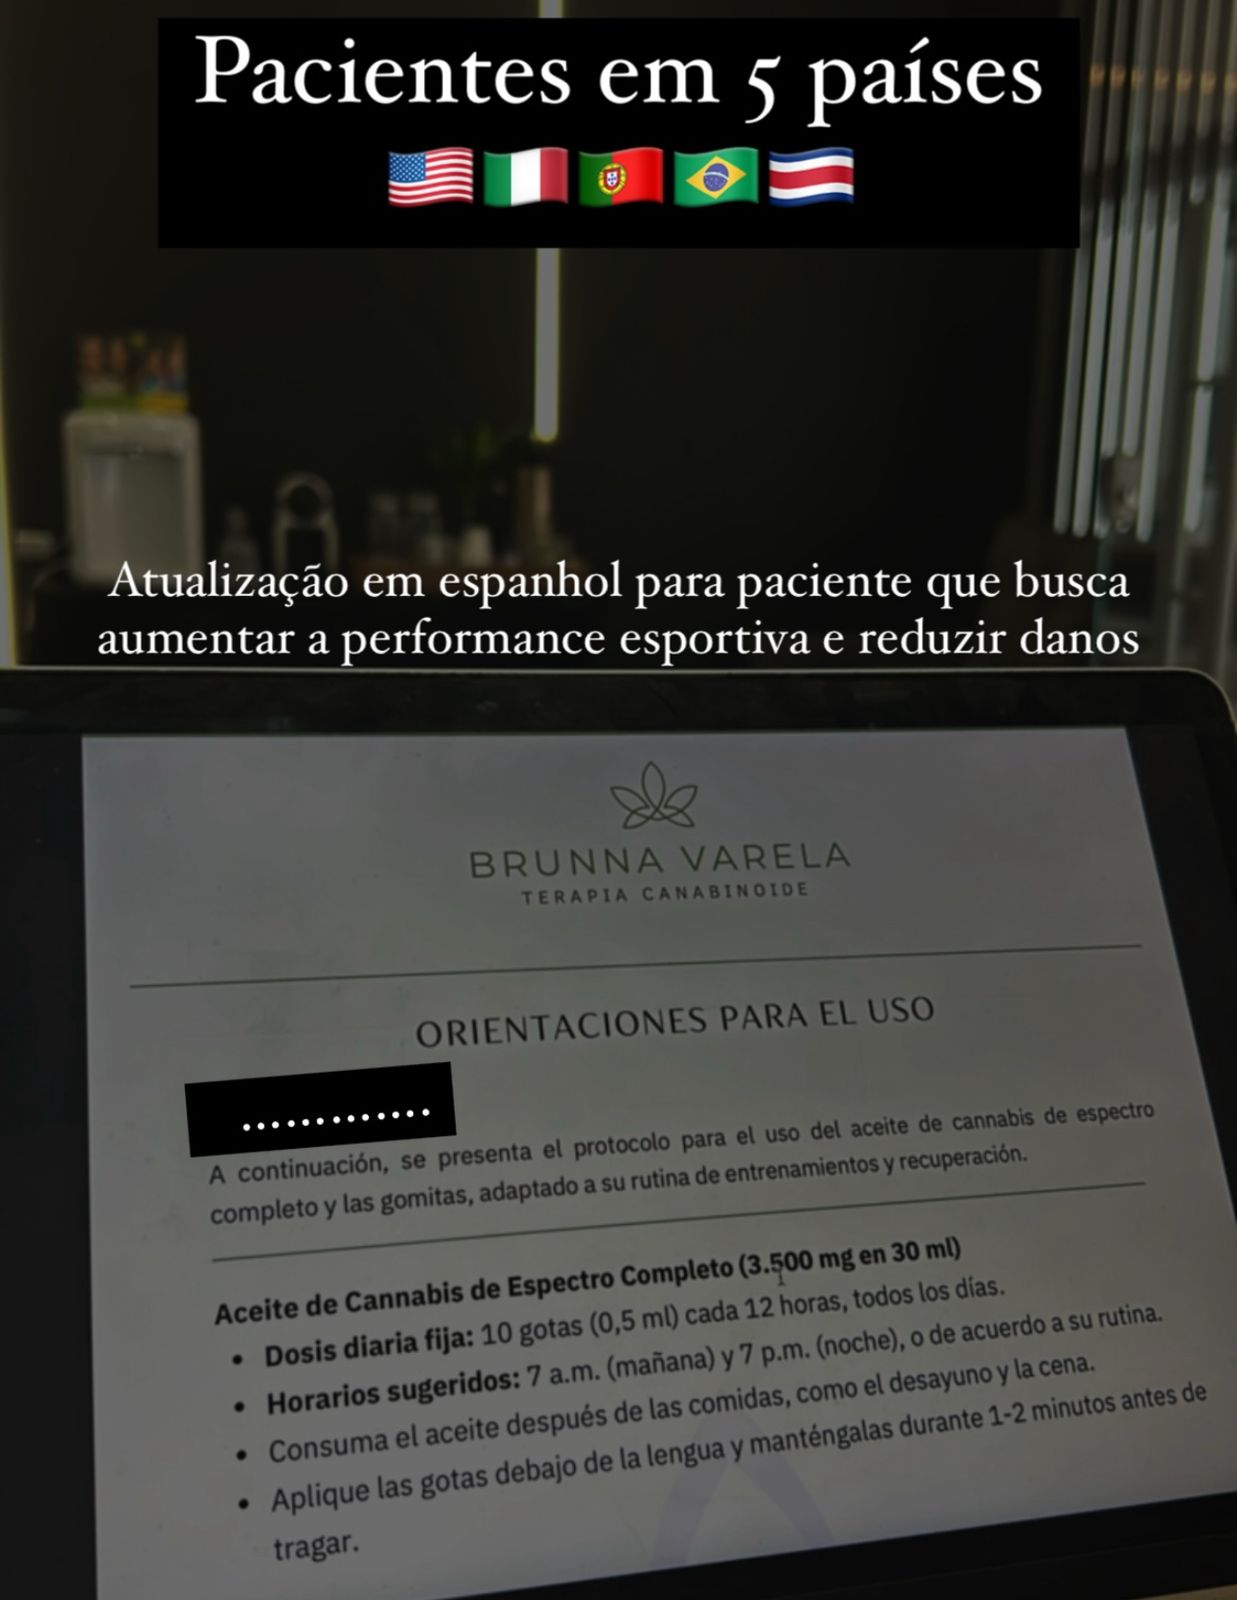
\includegraphics[width=0.4\linewidth]{imagens/linguagem.jpeg}
    \caption{Adaptação de idioma para pacientes estrangeiros. Registro do Autor (2025).}
    \label{fig:linguagem.png}
\end{figure}

Destaca-se também a importância de o novo sistema oferecer suporte multilíngue. O Instituto EDMA atende, ainda que em menor escala, pacientes internacionais. Dessa forma, é essencial que o sistema permita o acompanhamento do tratamento em diferentes idiomas, tanto na interface do paciente quanto nas comunicações automatizadas (como lembretes, formulários e orientações clínicas). A implementação de um sistema multilíngue contribuirá para garantir que todas as instruções e registros terapêuticos sejam compreendidos integralmente.

\begin{table}[H]
\centering
\caption{Necessidades e observações identificados a partir da entrevista com a profissional prescritora.}
\rowcolors{2}{gray!10}{white}
\begin{tabularx}{\textwidth}{|>{\raggedright\arraybackslash}p{4.2cm}|>{\raggedright\arraybackslash}X|}
\hline
\rowcolor{gray!20}
\textbf{Necessidade} & \textbf{Observações} \\
\hline
Formulário de anamnese automatizado & Envio automático após o primeiro contato do paciente, com integração direta ao prontuário eletrônico. \\
\hline
Escalas clínicas padronizadas & Envio e aplicação de escalas como Hamilton, Mini-Mental, Pittsburgh e BPI, conforme o perfil e a condição do paciente. \\
\hline
Acompanhamento semanal automatizado & Sistema deve enviar formulários semanalmente por 90 dias, com registro da evolução, para facilitar o ajuste da dose. \\
\hline
Registro de sintomas e doses & Aplicativo/sistema deve permitir ao paciente inserir sintomas, efeitos adversos e alterações de dose, com integração automática ao prontuário. \\
\hline
Dashboards e gráficos clínicos & Visualização clara da evolução clínica (ex: sono, dor, humor) por meio de gráficos automáticos. \\
\hline
Agenda integrada & Integração entre a agenda de atendimento e os acompanhamentos planejados, com alertas automáticos. \\
\hline
Automação do prontuário & Dados do formulário e acompanhamento devem ser integrados automaticamente ao prontuário, eliminando retrabalho. \\
\hline
Exportação de dados para pesquisa & Possibilidade de exportar dados clínicos e de acompanhamento (anonimizados) para fins de pesquisa científica. \\
\hline
Padronização para estudos científicos & Estruturação dos dados clínicos visando uso posterior para subgrupos, artigos e evidências de mundo real. \\
\hline
Registro do produto prescrito & Deve conter tipo de produto (isolado, broad, full), marca, lote, concentração, e histórico de alterações. \\
\hline
Controle de ajuste de dose & Histórico de ajustes, datas, justificativas, inclusive casos de desmame, deve ser documentado de forma estruturada. \\
\hline
Interface multilíngue & O sistema deve ser acessível em português, inglês e espanhol, considerando pacientes internacionais. \\
\hline
Backup e segurança de dados & Backup automático, com conformidade com LGPD e normas da Anvisa; dados criptografados. \\
\hline
Comunicação com pacientes & Integração com canais como WhatsApp ou chat interno para manter contato e orientar o paciente entre as consultas. \\
\hline
Controle de acesso por perfil & Diferenciar permissões entre prescritores, equipe técnica e pacientes, garantindo privacidade e segurança. \\
\hline
Interface responsiva e amigável & Suporte a celular e computador, com foco em facilidade de uso para pacientes e profissionais. \\
\hline
\end{tabularx}
\end{table}




Em relação à familiaridade com tecnologias, a maior parte dos pacientes classificou sua facilidade de uso entre níveis intermediário e avançado, sendo unânime a preferência pelo uso de dispositivos móveis para acesso ao sistema. Portanto, a prioridade deverá ser o desenvolvimento de uma interface responsiva, com foco na usabilidade em smartphones, sem prejuízo à compatibilidade com computadores e tablets.

\begin{table}[H]
\centering
\caption{Necessidades e observações identificados a partir da entrevista com os pacientes.}
\rowcolors{2}{gray!10}{white}
\begin{tabularx}{\textwidth}{|>{\raggedright\arraybackslash}p{4.2cm}|>{\raggedright\arraybackslash}X|}
\hline
\rowcolor{gray!20}
\textbf{Necessidades} & \textbf{Observações} \\
\hline
Lembretes de dose & Pacientes relataram dificuldade para lembrar de tomar as doses. A maioria demonstrou interesse em receber lembretes automatizados, preferencialmente via aplicativo ou WhatsApp. \\
\hline
Espaço para relatar efeitos entre consultas & Há grande interesse em um campo no sistema para relatar sintomas, efeitos adversos ou melhorias entre as consultas, facilitando o acompanhamento pela profissional prescritor(a). \\
\hline
Método de registro da evolução & A maioria prefere o uso de aplicativos móveis para acompanhar o tratamento. Alguns utilizam ferramentas improvisadas, como o Canva, e relataram dificuldade pela falta de um sistema específico para esse fim. \\
\hline
Compartilhamento de informações & Atualmente, o compartilhamento ocorre por meio de consultas presenciais, online e mensagens. Foi sugerida a integração do sistema com canais de comunicação como o WhatsApp. \\
\hline
Facilidade com tecnologia & Os pacientes entrevistados se autodeclaram com facilidade moderada a alta no uso de tecnologia, como aplicativos e sistemas digitais. \\
\hline
Dispositivo preferido de acesso & A maioria dos participantes indicou preferência pelo uso de celular, embora haja quem utilize o computador ou ambos. \\
\hline
Funcionalidades desejadas & Entre as sugestões estão: registros intuitivos, gráficos de evolução do tratamento, histórico de sintomas, lembretes, e um sistema que substitua o uso improvisado de ferramentas como o Canva. \\
\hline
\end{tabularx}
\end{table}


Com base nessas informações, conclui-se que o novo sistema deve contemplar uma abordagem centrada tanto nas necessidades operacionais do prescritor, quanto na experiência do paciente em tratamento. A implementação desse sistema pode otimizar o tempo clínico e favorecer o engajamento terapêutico, bem como contribuir com um cuidado mais efetivo e longitudinal.

\section{REQUISITOS}

\subsection{Requisitos funcionais do sistema}

\begin{table}[H]
\centering
\caption{Tabela de Requisitos Funcionais do Sistema}
\rowcolors{2}{gray!10}{white}
\begin{tabularx}{\textwidth}{|>{\raggedright\arraybackslash}p{1cm}|>{\raggedright\arraybackslash}p{2.5cm}|>{\raggedright\arraybackslash}p{2cm}|>{\raggedright\arraybackslash}X|}
\hline
\rowcolor{gray!20}
\textbf{ID} & \textbf{Requisito} & \textbf{Usuário} & \textbf{Descrição}\\
\hline
RF01 & Login & Paciente; Prescritor & Acesso ao sistema inserindo e-mail e senha previamente cadastrados. O sistema validará essas credenciais e, em caso de sucesso, redirecionará o usuário para a tela inicial, personalizada conforme seu perfil.\\
\hline
RF02 & Cadastrar usuário & Paciente; Prescritor & O usuário deverá preencher um formulário com campos obrigatórios, como nome completo, CPF, e-mail, data de nascimento, telefone e endereço.\\
\hline
RF03 & Tela Inicial (Dashboard) & Paciente; Prescritor & Após o login, o usuário será direcionado à sua tela inicial, onde poderá visualizar informações personalizadas, como consultas futuras, status de formulários, notificações de alertas clínicos e outras atividades relevantes.\\
\hline
RF04 & Consulta Clínica & Prescritor & Durante a consulta, o prescritor poderá acessar a ficha clínica do paciente, onde irá registrar observações sobre a condição do paciente. A ficha clínica será atualizada e estará disponível para consultas futuras.\\
\hline
RF05 & Prescrição & Prescritor & A prescrição será feita de forma digital, onde o prescritor poderá definir a formulação, a concentração do óleo, a dosagem, a frequência e quaisquer instruções específicas relacionadas ao tratamento. O sistema também permitirá a revisão e modificação de prescrições conforme necessário.\\
\hline
RF06 & Tela de Acompanhamento & Paciente & O paciente deverá acessar semanalmente a tela de acompanhamento para registrar a evolução do tratamento. Nessa tela, ele poderá responder a questionários sobre seu estado clínico, registrar sintomas, e outras informações pertinentes à sua condição de saúde.\\
\hline
RF07 & Tela de Acompanhamento & Prescritor & O prescritor poderá visualizar a evolução clínica do paciente através de gráficos, tabelas e comentários inseridos pelo próprio paciente, organizados por datas.\\
\hline
RF08 & Tela de Escalas Clínicas & Paciente & O paciente terá acesso a escalas clínicas padronizadas, onde ele poderá responder a questões que avaliam seu estado clínico atual.\\
\hline
\end{tabularx}
\end{table}

\newpage

\begin{table}[H]
\centering
\rowcolors{2}{gray!10}{white}
\begin{tabularx}{\textwidth}{|>{\raggedright\arraybackslash}p{1cm}|>{\raggedright\arraybackslash}p{3cm}|>{\raggedright\arraybackslash}p{2cm}|>{\raggedright\arraybackslash}X|}
\hline
\rowcolor{gray!20}
\textbf{ID} & \textbf{Requisito} & \textbf{Usuário} & \textbf{Descrição}\\
\hline
RF09 & Tela de Escalas Clínicas & Prescritor & O prescritor poderá cadastrar ou atualizar escalas clínicas ou selecionar escalas padronizadas existentes para disponibilizar aos pacientes.\\
\hline
RF10 & Tela de Agendamento & Paciente & O paciente poderá agendar suas consultas diretamente no sistema, visualizando a disponibilidade dos prescritores e escolhendo horários adequados. O sistema enviará notificações automáticas de lembretes.\\
\hline
RF11 & Tela de Agendamento & Prescritor & O prescritor poderá agendar consultas para seus pacientes, com visualização de sua agenda. O sistema permitirá gerenciar e editar a agenda, além de enviar notificações para o paciente sobre alterações no agendamento.\\
\hline
RF12 & Tela de Histórico Clínico & Paciente & O paciente poderá acessar e visualizar seu histórico clínico completo, que incluirá dados como anamnese, diagnósticos realizados, tratamentos prescritos, evoluções no quadro clínico, e quaisquer prescrições anteriores. A sistema permitirá também a exportação desses dados.\\
\hline
RF13 & Tela de Histórico Clínico & Prescritor & O prescritor terá acesso completo ao histórico clínico do paciente, podendo consultar todas as informações relacionadas a tratamentos passados, diagnósticos e prescrições.\\
\hline
RF14 & Tela de Notificações & Paciente & O paciente será notificado sobre compromissos agendados, alertas de consultas e formulários pendentes. As notificações podem ser configuradas conforme a preferência do paciente.\\
\hline
RF15 & Tela de Notificações & Prescritor & O prescritor será notificado sobre compromissos agendados, novos registros de pacientes, formulários preenchidos e outras ações importantes.\\
\hline
RF16 & Tela de Relatórios & Paciente & O paciente poderá gerar relatórios sobre o seu progresso clínico, incluindo dados sobre sintomas, evolução do quadro, e outros indicadores de saúde. O sistema permitirá que esses relatórios sejam exportados ou impressos, para que o paciente os leve a outras consultas\\
\hline
RF17 & Tela de Relatórios & Prescritor & O prescritor poderá gerar relatórios sobre a evolução clínica de seus pacientes, incluindo informações como diagnósticos, tratamentos anteriores e resultados obtidos.\\
\hline
RF18 & Tela de Configurações & Paciente; Prescritor & O usuário poderá alterar suas informações pessoais, como dados de contato e preferências de notificação.\\
\hline
\end{tabularx}
\end{table}

\subsection{Requisitos não funcionais do sistema}
\begin{table}[H]
\centering
\caption{Tabela de Requisitos Não Funcionais do Sistema}
\rowcolors{2}{gray!10}{white}
\begin{tabularx}{\textwidth}{|>{\raggedright\arraybackslash}p{1.5cm}|>{\raggedright\arraybackslash}p{3cm}|>{\raggedright\arraybackslash}p{3cm}|>{\raggedright\arraybackslash}X|}
\hline
\rowcolor{gray!20}
\textbf{ID} & \textbf{Requisito} & \textbf{Categoria} & \textbf{Descrição}\\
\hline
RNF14 & Usabilidade & Usabilidade & O sistema deve oferecer uma interface simples e de fácil navegação, adequada para usuários com diferentes níveis de familiaridade com tecnologia.\\
\hline
RNF15 & Usabilidade & Usabilidade & As telas devem ser responsivas e adaptáveis a dispositivos móveis e desktop, garantindo acessibilidade em diferentes resoluções.\\
\hline
RNF16 & Controle de Permissões & Segurança & O sistema deve garantir controle de acesso baseado em perfis, permitindo visualização e edição apenas conforme a permissão atribuída.\\
\hline
RNF17 & LGPD & Segurança & Todas as ações que envolvam dados sensíveis devem estar em conformidade com a Lei Geral de Proteção de Dados Pessoais (LGPD).\\
\hline
RNF18 & Tempo de Resposta & Desempenho & As principais funcionalidades, como login, consulta, prescrição e acompanhamento, devem apresentar tempo de resposta inferior a 3 segundos em rede estável.\\
\hline
RNF19 & Backup & Confiabilidade & O sistema deve realizar backups automáticos diários para evitar perda de dados clínicos e administrativos.\\
\hline
RNF20 & Adição de Funcionalidades & Extensibilidade & Deve ser possível incluir novas escalas clínicas, campos nos formulários e ajustes no fluxo sem a necessidade de reescrever partes centrais do sistema.\\
\hline
RNF21 & Compatibilidade com Sistemas & Interoperabilidade & O sistema deve ser compatível com exportação de dados em formatos abertos como PDF e CSV, além de permitir integração futura com sistemas como o Amplimed.\\
\hline
RNF22 & Integração com Comunicação & Conectividade & Deve haver suporte à integração com ferramentas externas de comunicação.\\
\hline
\end{tabularx}
\end{table}

\end{document}